\PassOptionsToPackage{subsection=false}{beamerouterthememiniframes}
\PassOptionsToPackage{dvipsnames,table}{xcolor}
\documentclass[fleqn]{beamer}
\usepackage{graphicx}
\usepackage{multirow}
\usepackage{multicol}
\usepackage{amsmath,amsfonts,amsthm,amsopn}
\usepackage{color, colortbl}
\usepackage{subfig}
\usepackage{wrapfig}
\usepackage{fancybox}
\usepackage{tikz}
\usepackage{fancyhdr}
\usepackage{setspace}
\usepackage{xcolor}
\usepackage{movie15}
\usepackage{pifont}
\usepackage{soul}
\usepackage{fancyvrb,newverbs}
\usepackage{epsfig}
\usepackage{epstopdf}
\fvset{fontsize=\footnotesize}
\RecustomVerbatimEnvironment{verbatim}{Verbatim}{}

%\usepackage{fancybox}

\usetheme{Szeged}
\usecolortheme{default}

%\definecolor{links}{HTML}{2A1B81}
%\definecolor{links}{blue!20}
\hypersetup{colorlinks,linkcolor=,urlcolor=blue!80}

\setbeamertemplate{blocks}[rounded]
\setbeamercolor{block title}{bg=blue!40,fg=black}
\setbeamercolor{block body}{bg=blue!10}


\newenvironment<>{clicker}[1]{%
  \begin{actionenv}#2%
      \def\insertblocktitle{#1}%
      \par%
      \mode<presentation>{%
        \setbeamercolor{block title}{fg=white,bg=magenta}
       \setbeamercolor{block body}{fg=black,bg=magenta!10}
       \setbeamercolor{itemize item}{fg=magenta}
       \setbeamertemplate{itemize item}[triangle]
       \setbeamercolor{enumerate item}{fg=magenta}
     }%
      \usebeamertemplate{block begin}}
    {\par\usebeamertemplate{block end}\end{actionenv}}

%\newcommand{\bmp}{\begin{minipage}}
%\newcommand{\emp}{\end{minipage}}
%\newcommand{\blankcolumn}{\bmp{.05\textwidth}\hspace{0.50in} \emp}

\defbeamertemplate*{footline}{infolines theme}
{
  \leavevmode%
  \hbox{%
  \begin{beamercolorbox}[wd=.333333\paperwidth,ht=2.25ex,dp=1ex,left]{author in head/foot}%
    \usebeamerfont{author in head/foot}~~\insertshortinstitute: \insertshorttitle
  \end{beamercolorbox}%
  \begin{beamercolorbox}[wd=.67\paperwidth,ht=2.25ex,dp=1ex,right]{date in head/foot}%
    \usebeamerfont{date in head/foot}%\insertshortdate{}\hspace*{2em}
    \insertframenumber{} / \inserttotalframenumber\hspace*{2ex}
  \end{beamercolorbox}
  }%
  \vskip0pt%
}

\newcommand{\cmark}{\ding{51}}%
\newcommand{\xmark}{\ding{55}}%
\newcommand{\grp}{\textcolor{magenta}{Group Exercise}}
\newcommand{\grpc}{\textcolor{magenta}{Group Exercise, continued}}
\newcommand{\bsans}[1]{\underline{\hspace{0.2in}\color{blue!80}{#1}\hspace{0.2in}}}

\definecolor{cverbbg}{gray}{0.93}
\newenvironment{cverbatim}
 {\SaveVerbatim{cverb}}
 {\endSaveVerbatim
  \flushleft\fboxrule=0pt\fboxsep=.5em
  \colorbox{cverbbg}{\BUseVerbatim{cverb}}%
  \endflushleft
}
\newenvironment{lcverbatim}
 {\SaveVerbatim{cverb}}
 {\endSaveVerbatim
  \flushleft\fboxrule=0pt\fboxsep=.5em
  \colorbox{cverbbg}{%
    \makebox[\dimexpr\linewidth-2\fboxsep][l]{\BUseVerbatim{cverb}}%
  }
  \endflushleft
}

\newcommand{\bmp}{\begin{minipage}}
\newcommand{\emp}{\end{minipage}}
\newcommand{\blankcolumn}{\bmp{.05\textwidth}\hspace{0.50in} \emp}

 \newenvironment{code}[1]%
  {\vspace{.1in}\footnotesize\Verbatim[frame=single,label=SAS Code,commandchars=\\\{\},xrightmargin=#1\textwidth,framesep=.2in,labelposition=all]}
  {\endVerbatim\normalsize}

 \newenvironment{Rcode}[1]%
  {\vspace{.1in}\footnotesize\Verbatim[frame=single,label=R Code,commandchars=\\\{\},xrightmargin=#1\textwidth,framesep=.2in,labelposition=all]}
  {\endVerbatim\normalsize}

   \newenvironment{RcodeScript}[1]%
  {\vspace{.1in}\scriptsize\Verbatim[frame=single,label=R Code,commandchars=\\\{\},xrightmargin=#1\textwidth,framesep=.2in,labelposition=all]}
  {\endVerbatim\normalsize}

 \newenvironment{RcodeTiny}[1]%
  {\vspace{.1in}\tiny\Verbatim[frame=single,label=R Code,commandchars=\\\{\},xrightmargin=#1\textwidth,framesep=.2in,labelposition=all]}
  {\endVerbatim\normalsize}


   \newenvironment{Rout}[1]%
  {\vspace{.1in}\footnotesize\Verbatim[frame=single,label=R Output,commandchars=\\\{\},xrightmargin=#1\textwidth,framesep=.2in,labelposition=all]}
  {\endVerbatim\normalsize}
  
     \newenvironment{MTout}[1]%
  {\vspace{.1in}\footnotesize\Verbatim[frame=single,label=Minitab Output,commandchars=\\\{\},xrightmargin=#1\textwidth,framesep=.2in,labelposition=all]}
  {\endVerbatim\normalsize}

   \newenvironment{RoutScript}[1]%
  {\vspace{.1in}\scriptsize\Verbatim[frame=single,label=R Output,commandchars=\\\{\},xrightmargin=#1\textwidth,framesep=.2in,labelposition=all]}
  {\endVerbatim\normalsize}

 \newenvironment{RoutTiny}[1]%
  {\vspace{.1in}\tiny\Verbatim[frame=single,label=R Output,commandchars=\\\{\},xrightmargin=#1\textwidth,framesep=.2in,labelposition=all]}
  {\endVerbatim\normalsize}

\newenvironment{craw}[2]%
{\vspace{.1in}\footnotesize\Verbatim[frame=single,label=#2,commandchars=\\\{\},xrightmargin=#1\textwidth,framesep=.2in,labelposition=all]}
  {\endVerbatim\normalsize}


\newenvironment{scriptcraw}[2]%
{\vspace{.1in}\scriptsize \Verbatim[frame=single,label=#2,commandchars=\\\{\},xrightmargin=#1\textwidth,framesep=.2in,labelposition=all]}
  {\endVerbatim\normalsize}

  \newenvironment{tinycraw}[2]%
{\vspace{.1in}\tiny \Verbatim[frame=single,label=#2,commandchars=\\\{\},xrightmargin=#1\textwidth,framesep=.2in,labelposition=all]}
  {\endVerbatim\normalsize}




\title[Set 8]{Regression models for time to event data}
\author[Pileggi]{Shannon Pileggi}

\institute[STAT 417]{STAT 417}

\date{}


\begin{document}

\begin{frame}
\titlepage
\end{frame}

\begin{frame}
\frametitle{OUTLINE\qquad\qquad\qquad} \tableofcontents[hideallsubsections]
\end{frame}


%===========================================================================================================================
\section[Overview]{Overview}
%===========================================================================================================================
\subsection{}

\begin{frame}
\frametitle{Regression models for time to event data}
\begin{itemize}
\item In the Veterans Administration lung cancer example, we investigated differences in the survival experiences for individuals with various types of lung cancer.  Basically, we are addressing:
\item[]
\item[]
\item[]
%Lung cancer Survival rates depends on which type of cancer an individual has.
\item In addition, are there other \textbf{explanatory variables} (i.e. \textbf{predictors}), that are associated with the risk of dying from lung cancer?
%\vskip .6in
%treatment, diet, smoking status, etc.
\item To investigate the effects of predictor variables (\textbf{categorical} and \textbf{quantitative}) on the time to experience the event of interest (or some function of $T$) we can fit regression models to the time to event data.
%\item The idea is similar to using linear regression to investigate the (partial) effects of independent variables $X_1,X_2, \ldots,X_p$ on a response variable $Y$.
%\item One important goal of survival
%analysis is to investigate the effects
%of explanatory variables on the ``risk" or ``potential" of experiencing a target
%event, similar to the goal of regression analysis.

%\item By constructing an appropriate model, we want to
%examine whether variation in the hazard can be explained by a set of predictors.
\end{itemize}
\end{frame}


\begin{frame}
\frametitle{Two approaches}
\begin{enumerate}

\item The \textbf{Cox regression model} (also referred to as the  \textbf{proportional hazards (PH) model}):
The hazard function $h(t)$ depends on a set of $p$ explanatory variables $X_1,X_2, \ldots,X_p$ through the model:
\item[]
\item[]
\item[]
%    \begin{eqnarray}
%    \boxed{h(t|X_1,X_2,\ldots,X_p)=h_0(t)\exp[\beta_1X_1+\beta_2X_2+\cdots+\beta_pX_p]} \nonumber
%    \end{eqnarray}
where $h_0(t)$ is called a \textit{baseline hazard function} that is assumed to be common for each subject.
%the h(t|$X_1,X_2,\ldots,X_p$) notation is to reinforce the dependence of the hazard on explanatory variables


%Expresses the dependence of the hazard function $h(t)$ as a linear combination of the natural log of a \textit{baseline} hazard function, $h_0(t)$, and the $p$ explanatory variables $X_1,X_2, \ldots,X_p$:
%    \begin{eqnarray}
%    \boxed{\ln[h(t|X_1,X_2,\ldots,X_p)]=\ln[h_0(t)]+\beta_1X_1+\beta_2X_2+\cdots+\beta_pX_p} \nonumber
%    \end{eqnarray}
%    which can also be re-expressed as:
%    \begin{eqnarray}
%    \boxed{h(t|X_1,X_2,\ldots,X_p)=h_0(t)\exp[\beta_1X_1+\beta_2X_2+\cdots+\beta_pX_p]} \nonumber
%    \end{eqnarray}
%Model the hazard function because it considers survival up to time t, takes into consideration the aging process
%of subjects

\item The \textbf{accelerated failure time (AFT) model}. Expresses the (natural) log of the time-to-event random variable $T$ as a linear combination of the $p$ explanatory variables $X_1,X_2, \ldots,X_p$:
\item[]
\item[]
\item[]
%    \begin{eqnarray}
%    {\ln(T)=\beta_0+\beta_1X_1+\beta_2X_2+\cdots+\beta_pX_p+\sigma W} \nonumber
%    \end{eqnarray}
    where $\sigma$ is a scale parameter and $W$ represents a random error term with some specific distribution.
%parametric because we must assume a distribution for the errors
%\item \textbf{Remark 1}: The response term in the Cox regression model is hazard, while in the AFT model, the response term is (a function of) the time-to-event random variable $T$.

%\item \textbf{Remark}: In both models, $\beta_1,\ldots,\beta_p$ represent parameters that must be estimated.
\end{enumerate}
\end{frame}


\begin{frame}
\frametitle{Why model hazard?}
\begin{enumerate}
\item
\item[] %Hazard assesses risk (of experiencing the event) at time $t$ \textit{conditional} on survival to time $t$, so the model takes into account the ``aging" of subjects, i.e. the subject has survived to a particular time $t$.
\item[] %survival is an unconditional prob
\item[]
\item %Interpretation of the results is fairly straightforward.
\item[]
\item[]
\item[]
\item % The development of the CR models is extensive and CR models are widely used in applications.
\item[]
\item[]
\item[]
\end{enumerate}
\end{frame}


\begin{frame}
\frametitle{Goals of a Cox regression model}
\begin{enumerate}
\item %Determine which variables are significantly associated with hazard (risk) of experiencing the event
\item[]
\item[]
\item[]
\item %Interpret the effects of the variables on hazard
\item[]
\item[]
\item[]
\item %Estimate survival and hazard rates for subjects controlling for values of the predictors
\item[]
\item[]
\item[]
\end{enumerate}
\end{frame}


%===========================================================================================================================
\section[CR: one categorical predictor]{CR: one categorical predictor}
%===========================================================================================================================
\subsection{}
\begin{frame}
\tableofcontents[currentsection, hideallsubsections]
\end{frame}

\begin{frame}
\frametitle{College graduation data}
How long does it take for students to graduate from college?  At what time(s) during their college career are they most likely to graduate?  How do graduation experiences vary by gender?
\begin{itemize}
\item Using data on a sample of 1000 participants from the National Educational Longitudinal Survey (NELS) from 1988-2002, we will investigate whether student's gender has an effect on the time required to obtain a bachelor's degree.
%\item Note that this sample includes individuals who began any community college or bachelor's granting post-secondary institution.
%So some students who began their post-secondary education at a two-year college may not have been intending to pursue a bachelor's degree.
\item Let $T=$ time (in months) taken to complete the requirements for a bachelor's degree.
\item If an individual had pursued and obtained a bachelor's degree by the interview date (in 2000), then her/his
event time is complete. If the student dropped out or did not graduate by the date they were interviewed, then her/his time is right censored.
\end{itemize}
\end{frame}

\begin{frame}
\frametitle{KM curves: years until graduation}
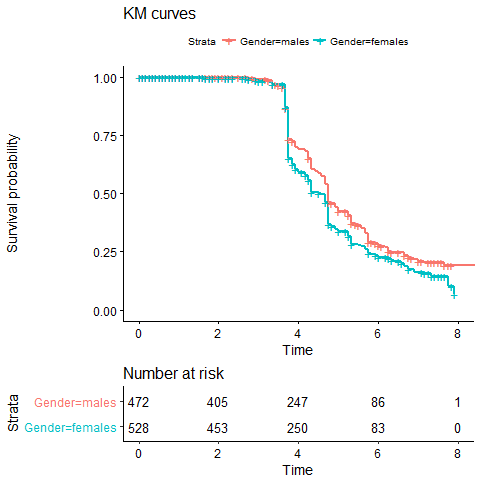
\includegraphics[width=0.6\textwidth]{Figures/KM_grad_surv.png}
% curve for males always above curve for females - don't intersect
\end{frame}

\begin{frame}
\frametitle{$\tilde{H}(t)$: years until graduation}
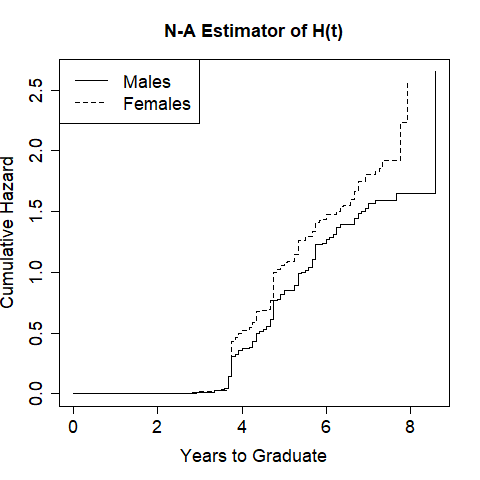
\includegraphics[width=0.6\textwidth]{Figures/KM_cumhaz_surv.png}
% females accumulate hazard at a faster rate than males; BUT ratio of CH  for female to CH of male is approx
% equal at all time t
\end{frame}

\begin{frame}
\frametitle{$\ln[\tilde{H}(t)]$: years until graduation}
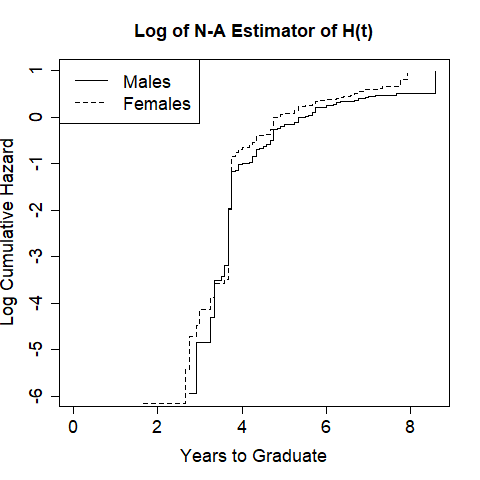
\includegraphics[width=0.6\textwidth]{Figures/KM_logcumhaz_surv.png}
%distance between curves constant across all time t
\end{frame}


\begin{frame}
\frametitle{Cox regression model: one categorical predictor}
Let's set up a CR model with one dichotomous (categorical) predictor, $X$, that only takes values 0 or 1.  The form of the CR model is:
\vskip200pt
\end{frame}


\begin{frame}
\frametitle{Cox regression model: one categorical predictor}
Let \texttt{X = 1} for females and \texttt{X = 0} for males.  Find the ratio of the hazard functions for females to males.
\vskip200pt
\end{frame}

\begin{frame}
\frametitle{Back to the picture...}
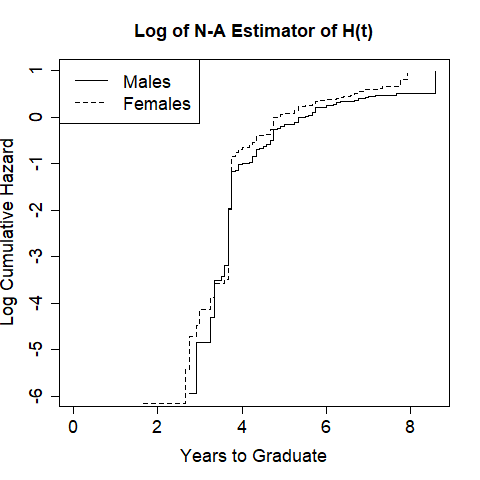
\includegraphics[width=0.5\textwidth]{Figures/KM_logcumhaz_surv.png}
%distance between curves constant across all time t
\end{frame}

%===========================================================================================================================
\section[Proportionality]{Proportionality}
%===========================================================================================================================
\subsection{}
\begin{frame}
\tableofcontents[currentsection, hideallsubsections]
\end{frame}

\begin{frame}
\frametitle{Example of proportionality}
Suppose that the CR model is given by:
\begin{eqnarray}
h(t|X) = \frac{(1.6)t^{.6}}{(5.74)^{1.6}}e^{.5X} \nonumber
\end{eqnarray}
where $X=1$ indicates membership to Group 1, and $X=0$ indicates membership to Group 2.
\begin{enumerate}
\item[]
\item What is the baseline hazard function? What is the value of the parameter $\beta$?
\end{enumerate}
\vskip200pt
\end{frame}

\begin{frame}
\frametitle{Example of proportionality}
\bmp{0.5\textwidth}
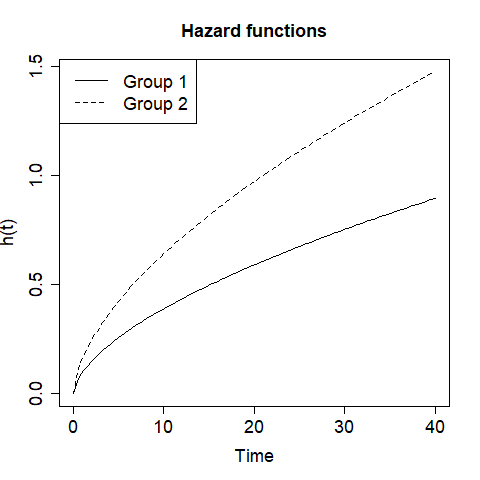
\includegraphics[width=1.0\textwidth]{Figures/prop_haz_groups.png}\\
\vskip30pt
\textcolor{white}{e}
\emp
\blankcolumn
\bmp{0.5\textwidth}
\begin{enumerate}
\setcounter{enumi}{1}
\item Show that the ratio of the hazard functions (hazard ratio) of Group 1 to Group 2 is constant across time $t$.
\end{enumerate}
\vskip200pt
\textcolor{white}{e}
\emp
\end{frame}

\begin{frame}
\frametitle{Example of proportionality}
\bmp{0.5\textwidth}
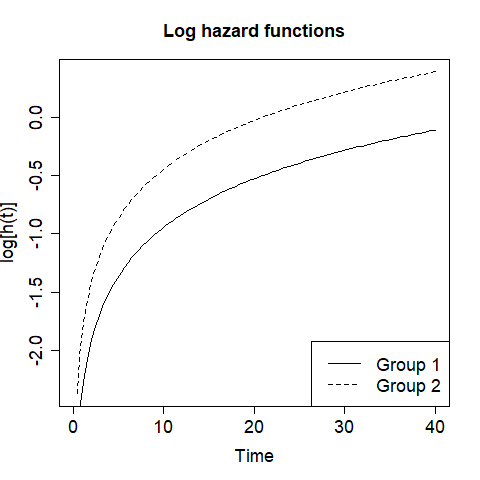
\includegraphics[width=1.0\textwidth]{Figures/prop_loghaz_groups.png}\\
\vskip30pt
\textcolor{white}{e}
\emp
\blankcolumn
\bmp{0.5\textwidth}
\begin{enumerate}
\setcounter{enumi}{2}
\item Show that the difference in the log-hazard functions between Group 1 and Group 2 is constant across time $t$.
\end{enumerate}
\vskip200pt
\textcolor{white}{e}
\emp
\end{frame}


\begin{frame}
\frametitle{CR model: proportionality assumption}
The main feature about the CR models observed in the above examples is known as the \textit{proportionality assumption}.  In general, for a set of $p$ explanatory variables $X_1,X_2,\ldots,X_p$, the \textbf{hazard ratio (HR)} is given by:
\vskip200pt
%\begin{itemize}
%\item The ratio of the hazard function for an individual with fixed values of the explanatory variables to the hazard function for another individual with fixed values of the explanatory variables is constant across time:
%\vskip 1in
%%The ratio of the two hazard functions will be constant over time
%%h(t|x1,x2,...,xp)/h(t|x1*,x2*,...,xp*) = exp[B1(x1-x1*)+...+Bp(xp-xp*)]

%This ratio is commonly referred to as the \textbf{hazard ratio} and \textit{does not} depend on time $t$.

%\item The proportionality assumption also implies that the \textit{difference} between the
%natural logs of the hazard functions will be constant over time.
%%ln[h(t|x1,x2,...,xp)]-ln[h(t|x1*,x2*,...,xp*)] = [B1(x1-x1*)+...+Bp(xp-xp*)]
%\end{itemize}
\end{frame}


%===========================================================================================================================
\section[Interpretations]{Interpretations}
%===========================================================================================================================
\subsection{}
\begin{frame}
\tableofcontents[currentsection, hideallsubsections]
\end{frame}

\begin{frame}
\frametitle{CR model: one categorical predictor}
Consider the CR model with one binary categorical predictor where $X$ takes the value 0 or 1:
$\displaystyle h(t|X) = h_0(t)e^{\beta X}$
\begin{itemize}
\item $\beta$ represents:
\item[]
\item[]
\item[]
% the difference between the \textit{natural logarithm} of the hazard
%functions for subjects with $X=1$ and subjects with $X=0$.
\item  $e^\beta$ is the \textbf{hazard ratio (HR)} and represents:
\item[]
\item[]
\item[]
\item[]
\item[]
%the multiplicative amount by which the rate of failure for individuals with X=1 differs from the
%rate of failure for individuals with X=0
\end{itemize}
\end{frame}

\begin{frame}
\frametitle{Interpretation of the hazard ratio $e^\beta$}
\hspace*{-0.3in}
\bmp{0.65\textwidth}
If $X$ is a categorical predictor taking values 0 or 1, then the hazard ratio ($HR$) of subjects with $X=1$ to subjects with $X=0$ is:
\emp
\bmp{0.35\textwidth}
\begin{eqnarray}
\boxed{HR = \frac{h(t|X=1)}{h(t|X=0)} = e^{\beta}} \nonumber
\end{eqnarray}
\emp
\begin{itemize}
\item $e^{\beta}>1$:
\item[]
\item[]
\item[]
%The hazard rate (rate of failure) for subj's with X=1 is e^{\beta} times higher than the hazard rate
%for subj's with X=0
\item $e^{\beta}<1$:
\item[]
\item[]
\item[]
%The hazard rate (rate of failure) for subj's with X=0 is e^{-\beta} times higher than the hazard rate
%for subj's with X=1
\item $e^{\beta}=1$:
\item[]
\item[]
\item[]
%The hazard rate (rate of failure) for subj's with X=1 is identical to the hazard rate
%for subj's with X=0
\end{itemize}
\end{frame}

\begin{frame}
\frametitle{Example interpretation}
Consider the CR model for the graduation data, and suppose that $\beta=.2$ (where $X=1$ for females and $X=0$ for males).  Then the CR model would be given by:
\vskip40pt
\begin{enumerate}
\item Interpret the value of the coefficient $\beta=.2$.
%\item Interpret the value of the hazard ratio of females to males.
\end{enumerate}
\vskip200pt
\end{frame}

\begin{frame}
\frametitle{Example interpretation, cont.}
\begin{enumerate}
\setcounter{enumi}{1}
%\item Interpret the value of the coefficient $\beta=.2$.
\item Interpret the value of the hazard ratio of females to males.
\end{enumerate}
\vskip200pt
\end{frame}

\begin{frame}
\frametitle{CR model: one quantitative predictor}
\begin{itemize}
\item \textbf{Veterans Administration Lung Cancer Group Study}.  Recall the lung cancer study to investigate the effects of two treatments on survival.  Another explanatory variable available is the \textit{Karnofsky performance score} which is used to quantify cancer patients' functional impairment. The Karnofsky performance score is measured on a 0-100 scale in increments of 10 with 0 indicating that the subject is dead, and 100 indicating that the subject shows no signs of the disease.

\item Then $X=$ Karnofsky performance score is a \textit{quantitative} variable.

\item Suppose we want to investigate the effect of patient's Karnofsky score on the risk (hazard) of dying from lung cancer.
\end{itemize}
\end{frame}

\begin{frame}
\frametitle{CR model: one quantitative predictor}
\bmp{0.60\textwidth}
Suppose $X$ is quantitative and consider the CR model:
\emp
\bmp{0.40\textwidth}
\begin{eqnarray}
\boxed{h(t|X) = h_0(t)e^{\beta X}} \nonumber
\end{eqnarray}
\emp
\begin{itemize}
\item The CR model for subjects with $X=a$ is:
\item[]
\item[]
\item[]
\item The CR model for subjects with $X=a+c$ is:
\item[]
\item[]
\item[]
\item Then the hazard ratio for subjects with $X=a+c$ to subjects with $X=a$ is:
\item[]
\item[]
\item[]
\end{itemize}
\end{frame}

\begin{frame}
\frametitle{CR model: one quantitative predictor interpretation of HR}
The hazard ratio $e^{c\beta}$ is the multiplicative change in the hazard rate for a $c$ unit increase in $X$, or alternatively, $\beta$ is the change in log hazard for a $c$ unit increase in $X$.
\begin{itemize}
\item $e^{\beta}>1$:
\item[]
\item[]
\item[]
%%The hazard rate is e^{\beta c} times higher for each c unit increase in X
\item $e^{\beta}<1$:
\item[]
\item[]
\item[]
%The hazard rate is e^{ - \beta c} times higher for each c unit decrease in X
\item $e^{\beta}=1$:
\item[]
\item[]
\item[]
%The hazard rate (rate of failure) for subj's with X=1 is identical to the hazard rate
%for subj's with X=0
\end{itemize}
\end{frame}

\begin{frame}
\frametitle{Example interpretation with quantitative predictor}
To investigate the effect of patient's Karnofsky score on the hazard of death from lung cancer, suppose we have the CR model:
\begin{eqnarray}
h(t|X) = h_0(t)e^{-.03X} \nonumber
\end{eqnarray}
\begin{enumerate}
\item Interpret $\beta=-.03$.
\end{enumerate}
\vskip200pt
\end{frame}

\begin{frame}
\frametitle{Example interpretation with quantitative predictor, cont.}
\begin{enumerate}
\setcounter{enumi}{1}
\item Interpret $\beta=-.03$ in terms of a 10 point increase in Karnofsky score.
\end{enumerate}
\vskip200pt
\end{frame}

\begin{frame}
\frametitle{Example interpretation with quantitative predictor, cont.}
\begin{enumerate}
\setcounter{enumi}{2}
\item Compute and interpret the hazard ratio for a 10 point increase in Karnofsky score.
\end{enumerate}
\vskip200pt
\end{frame}


%===========================================================================================================================
\section[Estimation]{Estimation}
%===========================================================================================================================
\subsection{}
\begin{frame}
\tableofcontents[currentsection, hideallsubsections]
\end{frame}

\begin{frame}
\frametitle{Parameter estimation}
\begin{itemize}
\item In the previous examples, values of the parameter $\beta$ were given for the CR model. However, parameters values are typically unknown and must be estimated from data.
\item Recall the form of the CR model with one explanatory variable:
\begin{eqnarray}
h(t|X) = h_0(t)e^{\beta X} \nonumber
\end{eqnarray}
\item If we wanted to fully specify all the unknown quantities, what would we need?
\vskip .4in
%h_0(t) and \beta
\item In general, the parameter $\beta$ (or several $\beta$'s) will be unknown, as well as the baseline hazard function $h_0(t)$.
\item But since we treat $h_0(t)$ as a \textit{nuisance parameter}, we are not interested in immediately estimating this quantity (however, we can estimate it after we estimate the $\beta$'s).
\end{itemize}
\end{frame}

\begin{frame}
\frametitle{Partial maximum likelihood}
\begin{itemize}
\item A procedure called \textbf{partial maximum likelihood} that does not require any specification of the baseline hazard function is used to estimate the $\beta$ parameters only.
\item Skipping the mathematical details, but some notes:
  \begin{itemize}
   \item Only subjects with complete event times will contribute terms to the (partial) likelihood function, and the likelihood function will only contain $\beta$ terms (no $h_0(t)$ terms).
  \item Using numerical methods, software obtains the $\beta$ value(s) that maximize the likelihood function.
  \item The estimates of $\beta_1, \beta_2, \ldots, \beta_p$ will be denoted by:
  \vskip .4in
  %\hat{\beta}_1, \hat{\beta}_p,
  \end{itemize}

\item {Partial maximum likelihood} is implemented in many statistical software packages, but not Minitab!  CR models will be fit to time-to-event data in \texttt{R}.
%\item The partial maximum likelihood procedure requires contributions only from subjects with complete event times, whereas a full maximum likelihood procedure requires a contribution from every subject.
\end{itemize}
\end{frame}

\begin{frame}[fragile]
\frametitle{Fitting CR model in \texttt{R}}
\begin{Rcode}{-.05}
CR_grad <- \textcolor{OrangeRed}{coxph}(Surv(Years, Censor) ~ as.factor(Gender),
                 data = graduate)
summary(CR_grad)
\end{Rcode}
\vskip5pt
\begin{Rout}{-.05}
  n= 1000, number of events= 614

                      coef exp(coef) se(coef)     z Pr(>|z|)
as.factor(Gender)1 0.20862   1.23197  0.08141 2.563   0.0104 *
---
Signif. codes:  0 ‘***’ 0.001 ‘**’ 0.01 ‘*’ 0.05 ‘.’ 0.1 ‘ ’ 1
\end{Rout}
\end{frame}


\begin{frame}
\frametitle{Example interpretation of parameter estimates}
\begin{enumerate}
\item State the \emph{estimated} Cox regression model.
\item[]
\item[]
\item Interpret the value of the estimated coefficient $\hat{\beta}$.
\item[]
\item[]
\item[]
\item[]
\item Interpret the value of the estimated hazard ratio of females to males.
\item[]
\item[]
\item[]
\item[]
\end{enumerate}
\end{frame}

\begin{frame}[fragile]
%\frametitle{Full \texttt{R} output}
\begin{Rout}{-.05}
Call:
coxph(formula = Surv(Years, Censor) ~ as.factor(Gender), data = graduate)

  n= 1000, number of events= 614

                      coef exp(coef) se(coef)     z Pr(>|z|)
as.factor(Gender)1 0.20862   1.23197  0.08141 2.563   0.0104 *
---
Signif. codes:  0 ‘***’ 0.001 ‘**’ 0.01 ‘*’ 0.05 ‘.’ 0.1 ‘ ’ 1

                   exp(coef) exp(-coef) lower .95 upper .95
as.factor(Gender)1     1.232     0.8117      1.05     1.445

Concordance= 0.53  (se = 0.012 )
Rsquare= 0.007   (max possible= 0.999 )
Likelihood ratio test= 6.61  on 1 df,   p=0.01016
Wald test            = 6.57  on 1 df,   p=0.01039
Score (logrank) test = 6.59  on 1 df,   p=0.01025
\end{Rout}
\end{frame}


\end{document} 